\subsection{Social-GAN}
\label{sec:social_gan}
% Generated by models/social_gan/handoff.py from audited results.
\providecommand{\SocialGanInsight}[1]{\csname social-gan:#1\endcsname}
\expandafter\def\csname social-gan:OneSampleADE\endcsname{0.835}
\expandafter\def\csname social-gan:BudgetReduction\endcsname{61}
\expandafter\def\csname social-gan:MaxSeedSD\endcsname{0.027}
\expandafter\def\csname social-gan:NoiseMaxFoldDelta\endcsname{+0.556}
\expandafter\def\csname social-gan:NoiseMinFoldDelta\endcsname{+0.342}
\expandafter\def\csname social-gan:UnivRuntime\endcsname{17.6}
\expandafter\def\csname social-gan:CleanSpeedViolationPct\endcsname{5.7}
\expandafter\def\csname social-gan:CleanCloseApproachPct\endcsname{87.6}
\expandafter\def\csname social-gan:FixedCleanMinADE\endcsname{1.015}
\expandafter\def\csname social-gan:FixedNoiseMinADE\endcsname{0.565}
\expandafter\def\csname social-gan:FailureMinADE\endcsname{4.692}
\expandafter\def\csname social-gan:FailureCoTargets\endcsname{15}
\expandafter\def\csname social-gan:FailureHeading\endcsname{174}
\expandafter\def\csname social-gan:ETHMinADE\endcsname{0.633}
\expandafter\def\csname social-gan:ETHMinFDE\endcsname{1.233}
\expandafter\def\csname social-gan:ETHMeanADE\endcsname{1.151}
\expandafter\def\csname social-gan:ETHMeanFDE\endcsname{2.415}
\expandafter\def\csname social-gan:ETHEnergy\endcsname{0.982}
\expandafter\def\csname social-gan:ETHDiversity\endcsname{0.805}
\expandafter\def\csname social-gan:HotelMinADE\endcsname{0.207}
\expandafter\def\csname social-gan:HotelMinFDE\endcsname{0.380}
\expandafter\def\csname social-gan:HotelMeanADE\endcsname{0.790}
\expandafter\def\csname social-gan:HotelMeanFDE\endcsname{1.658}
\expandafter\def\csname social-gan:HotelEnergy\endcsname{0.431}
\expandafter\def\csname social-gan:HotelDiversity\endcsname{1.033}
\expandafter\def\csname social-gan:UnivMinADE\endcsname{0.333}
\expandafter\def\csname social-gan:UnivMinFDE\endcsname{0.632}
\expandafter\def\csname social-gan:UnivMeanADE\endcsname{0.783}
\expandafter\def\csname social-gan:UnivMeanFDE\endcsname{1.641}
\expandafter\def\csname social-gan:UnivEnergy\endcsname{0.559}
\expandafter\def\csname social-gan:UnivDiversity\endcsname{0.753}
\expandafter\def\csname social-gan:Zara1MinADE\endcsname{0.233}
\expandafter\def\csname social-gan:Zara1MinFDE\endcsname{0.408}
\expandafter\def\csname social-gan:Zara1MeanADE\endcsname{0.766}
\expandafter\def\csname social-gan:Zara1MeanFDE\endcsname{1.567}
\expandafter\def\csname social-gan:Zara1Energy\endcsname{0.438}
\expandafter\def\csname social-gan:Zara1Diversity\endcsname{0.952}
\expandafter\def\csname social-gan:Zara2MinADE\endcsname{0.204}
\expandafter\def\csname social-gan:Zara2MinFDE\endcsname{0.362}
\expandafter\def\csname social-gan:Zara2MeanADE\endcsname{0.706}
\expandafter\def\csname social-gan:Zara2MeanFDE\endcsname{1.460}
\expandafter\def\csname social-gan:Zara2Energy\endcsname{0.383}
\expandafter\def\csname social-gan:Zara2Diversity\endcsname{0.917}


\paragraph{Model.}
We adapted the pooled Social GAN of Gupta et al.\ \cite{gupta2018socialgan}.
A shared LSTM encodes the displacements in each observed track. At the
forecast origin, a multilayer perceptron combines each neighbor's state
with its offset from the target. An elementwise maximum summarizes the
nearest twelve eligible neighbors within 6\,m. Each neighbor must have
eight positions available through the anchor. An empty neighborhood
contributes a zero vector.

The target state, pooled context and a Gaussian draw initialize the
decoder. At each step the decoder predicts a correction to the average
displacement over the last four input intervals. Integrating those
steps from the target input endpoint recovers metric coordinates.
A separate LSTM discriminator scores the history followed by either
a real or a generated future. The generator minimizes the RMS error
of the closest of twenty training draws plus a weighted adversarial
loss. The neighborhood limit, residual decoder, target discriminator
and shorter training budget are features of this implementation.

\paragraph{Verification.}
We selected one checkpoint per fold and seed by clean validation Energy
Score, then meanADE, then earlier epoch. We used that checkpoint for all
six conditions and reused the same Gaussian draws within each scene and
anchor across conditions. Regression tests removed target and neighbor
futures and changed cached derivatives without changing the inputs or
forecasts. Coordinate round-trip and isolated-target tests passed. The
shared audit checked 90 bundles against the ordered manifests, and a
local replay regenerated the six ETH seed 0 forecasts from its formal
checkpoint.

\paragraph{Clean forecasts.}
With \(K=20\), the best path after seeing the future averaged
\ModelMetric{social_gan}{clean_0}{min_ade_mean}\,m ADE. The mean error
over the twenty paths was \ModelMetric{social_gan}{clean_0}{mean_ade_mean}\,m.
Scoring only the first draw gave \SocialGanInsight{OneSampleADE}\,m ADE.
Scoring all twenty lowered the minimum by \SocialGanInsight{BudgetReduction}\%
on the same forecasts. This quantifies the benefit of searching a larger
sample set with access to the truth. The clean Energy Score was
\ModelMetric{social_gan}{clean_0}{energy_score_mean}\,m. Across the five
folds, the largest within-fold seed standard deviation for minADE was
\SocialGanInsight{MaxSeedSD}\,m.

\begin{table}[H]
\centering
\small
\caption{Clean Social-GAN errors and sample diversity in meters at \(K=20\).
Each fold row averages three training seeds. The last row weights folds equally.}
\label{tab:social_gan:clean}
\begin{tabular}{lrrrrrr}
\toprule
Holdout & minADE & minFDE & meanADE & meanFDE & Energy & Diversity \\
\midrule
ETH & \SocialGanInsight{ETHMinADE} & \SocialGanInsight{ETHMinFDE} & \SocialGanInsight{ETHMeanADE} & \SocialGanInsight{ETHMeanFDE} & \SocialGanInsight{ETHEnergy} & \SocialGanInsight{ETHDiversity} \\
Hotel & \SocialGanInsight{HotelMinADE} & \SocialGanInsight{HotelMinFDE} & \SocialGanInsight{HotelMeanADE} & \SocialGanInsight{HotelMeanFDE} & \SocialGanInsight{HotelEnergy} & \SocialGanInsight{HotelDiversity} \\
Univ & \SocialGanInsight{UnivMinADE} & \SocialGanInsight{UnivMinFDE} & \SocialGanInsight{UnivMeanADE} & \SocialGanInsight{UnivMeanFDE} & \SocialGanInsight{UnivEnergy} & \SocialGanInsight{UnivDiversity} \\
Zara1 & \SocialGanInsight{Zara1MinADE} & \SocialGanInsight{Zara1MinFDE} & \SocialGanInsight{Zara1MeanADE} & \SocialGanInsight{Zara1MeanFDE} & \SocialGanInsight{Zara1Energy} & \SocialGanInsight{Zara1Diversity} \\
Zara2 & \SocialGanInsight{Zara2MinADE} & \SocialGanInsight{Zara2MinFDE} & \SocialGanInsight{Zara2MeanADE} & \SocialGanInsight{Zara2MeanFDE} & \SocialGanInsight{Zara2Energy} & \SocialGanInsight{Zara2Diversity} \\
\midrule
Macro & \ModelMetric{social_gan}{clean_0}{min_ade_mean} & \ModelMetric{social_gan}{clean_0}{min_fde_mean} &
\ModelMetric{social_gan}{clean_0}{mean_ade_mean} & \ModelMetric{social_gan}{clean_0}{mean_fde_mean} &
\ModelMetric{social_gan}{clean_0}{energy_score_mean} & \ModelMetric{social_gan}{clean_0}{sample_diversity_mean} \\
\bottomrule
\end{tabular}
\end{table}

\paragraph{Corrupted histories.}
For 0.05, 0.10 and 0.20\,m noise, the paired meanADE changes were
\ModelMeanADEChange{social_gan}{noise_005},
\ModelMeanADEChange{social_gan}{noise_010} and
\ModelMeanADEChange{social_gan}{noise_020}\,m.
The change under 0.20\,m noise ranged from
\SocialGanInsight{NoiseMinFoldDelta} to \SocialGanInsight{NoiseMaxFoldDelta}\,m
across holdouts. Hiding one or two points changed meanADE by
\ModelMeanADEChange{social_gan}{missing_1} and
\ModelMeanADEChange{social_gan}{missing_2}\,m. These are paired differences
against clean input at the same checkpoint. At 0.20\,m noise, pairwise
sample diversity rose from \ModelMetric{social_gan}{clean_0}{sample_diversity_mean}
to \ModelMetric{social_gan}{noise_020}{sample_diversity_mean}\,m, while
Energy Score rose to \ModelMetric{social_gan}{noise_020}{energy_score_mean}\,m.
In the fixed ETH example,
minADE went from \SocialGanInsight{FixedCleanMinADE} to
\SocialGanInsight{FixedNoiseMinADE}\,m under 0.20\,m noise, even though
the aggregate meanADE increased.
In the largest clean minADE failure in Univ at seed 0, even the closest
draw missed by \SocialGanInsight{FailureMinADE}\,m. The net direction
of the recorded future differed from the observed history by
\(\SocialGanInsight{FailureHeading}^{\circ}\) (Figure~\ref{fig:social_gan:paths}).

\begin{figure}[H]
\centering
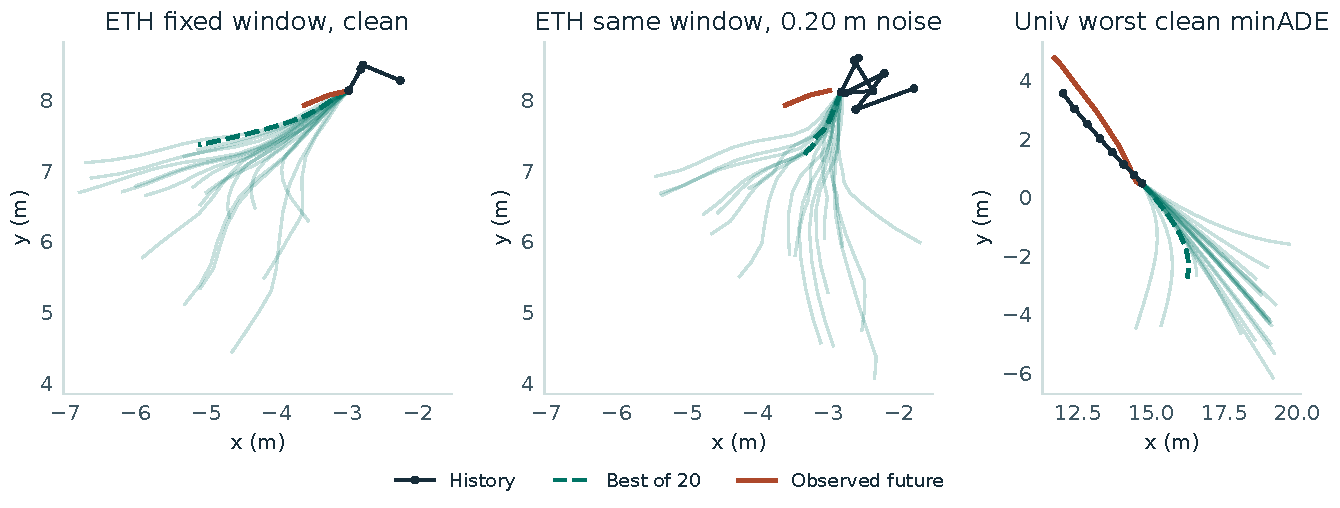
\includegraphics[width=\linewidth]{contributions/social_gan/assets/trajectory_examples.pdf}
\caption{Social-GAN samples and recorded futures at seed 0. The two ETH
panels use the same fixed window and latent draws. The Univ panel shows
the clean window with the largest minADE in that holdout and seed.}
\label{fig:social_gan:paths}
\end{figure}

\paragraph{Motion and runtime.}
On clean input, \SocialGanInsight{CleanSpeedViolationPct}\% of windows
had a forecast speed 99th percentile above the fold's training threshold.
The close-approach rate was \SocialGanInsight{CleanCloseApproachPct}\%,
averaged over draws and scene times with multiple targets. This pairs
equal sample indices across target-specific forecasts. The median of run
medians was \ModelRuntime{social_gan}{end_to_end_ms}\,ms
per 128 targets on an Apple M5 Pro CPU with two PyTorch threads
(\ModelRuntime{social_gan}{preprocessing_ms}\,ms for preprocessing and
\ModelRuntime{social_gan}{prediction_sampling_ms}\,ms for prediction and sampling).
Timing starts after one-time history indexing and ends at metric CPU
output. The results describe the complete model, with pooling, the
residual connection and the adversarial objective evaluated together.
